\documentclass[conference]{IEEEtran}
\IEEEoverridecommandlockouts

\usepackage{cite}
\usepackage{amsmath,amssymb,amsfonts}
\usepackage{graphicx}
\usepackage{textcomp}
\usepackage{xcolor}
\usepackage{booktabs}
\usepackage{array}
\usepackage{float}
\def\BibTeX{{\rm B\kern-.05em{\sc i\kern-.025em b}\kern-.08em
    T\kern-.1667em\lower.7ex\hbox{E}\kern-.125emX}}

\begin{document}

\title{Journal Recommendation System and Topic Clustering for Computer Science Articles\\
{\footnotesize Data Mining Final Project}}

\author{\IEEEauthorblockN{Ali Berk Ye\c{s}ilduman}
\IEEEauthorblockA{\textit{Computer Engineering Department}\\
\textit{Akdeniz University}\\
Student ID: 20200808035\\
Email: 20200808035@ogr.akdeniz.edu.tr\\
Final delivery regenerated from the accepted $K=46$ pipeline}
}

\maketitle

\begin{abstract}
This project implements a journal recommendation and topic clustering pipeline on the \textit{CompSciencePub.sqlite} database. The recommendation stage joins abstracts with author keywords, Web of Science subjects, and keyword plus fields, then ranks journals with a TF-IDF and cosine-similarity baseline. A leakage-free stratified 80/20 hold-out split over journals with at least five articles produced 28.37\% Top-1 accuracy, 45.89\% Top-3 accuracy, 54.96\% Top-5 accuracy, and 0.410 mean reciprocal rank on 4,596 held-out articles. For topic discovery, a domain-aware TF-IDF space was reduced with Truncated SVD and normalized before K-Means. Instead of choosing $K$ from a small local sweep, the final delivery analyzes $K=2..100$ with step 2 plus the manually compared $K=45$; in the current reproducible run, the Kneedle algorithm identifies $K=46$ as the elbow point. Although larger $K$ values achieve better scores on some individual metrics, the final submission keeps the $K=46$ K-Means model because it provides a balanced trade-off between clustering quality, model complexity, cluster-size distribution, and topic interpretability. An experimental BERTopic alternative was also evaluated with TF-IDF/SVD and sentence-transformer embeddings, but it was not selected for the final delivery because it depends on a heavier experimental stack and assigns a noticeable fraction of documents to outliers.
\end{abstract}

\begin{IEEEkeywords}
Data Mining, Text Mining, Recommender Systems, TF-IDF, K-Means, BERTopic, Topic Clustering
\end{IEEEkeywords}

\section{Introduction}
Selecting a suitable journal for a new manuscript is difficult because many journals overlap in topic, methodology, and audience. A practical journal finder should therefore rely on the manuscript content itself. In parallel, topic clustering can reveal the broad structure of the same literature collection and help explain how the corpus is organized.

The homework requires two core capabilities: recommending the top five journals for a user-provided abstract, and producing meaningful topic clusters from the provided computer science publication database. The final delivery also documents how the clustering decision was made, which alternatives were explored, and why the final method was preferred.

\section{Literature Review}
Academic journal recommendation is commonly modeled as a content-based retrieval problem. TF-IDF remains a strong baseline for scientific text, especially when abstracts are enriched with controlled metadata such as author keywords and subject terms \cite{cbf_recommender,metadata_nlp}. The ranking challenge is not only article retrieval but also journal-level aggregation of article similarities \cite{journal_scoring}.

For unsupervised topic discovery, K-Means is still attractive because it is fast, reproducible, and straightforward to interpret through cluster centroid terms. Truncated SVD is frequently paired with sparse text features to compress the term space while preserving major semantic structure \cite{kmeans_svd}. More recent topic-modeling pipelines such as BERTopic combine document embeddings, manifold learning, density-based clustering, and c-TF-IDF topic representations, but they often trade simplicity and determinism for additional flexibility.

\section{Methodology}
\subsection{Data Integration and Preprocessing}
The database tables \textit{AcademicRecord}, \textit{AcademicRecordAbstract}, and \textit{Publication} were joined to obtain article identifiers, abstracts, and journal names. Additional one-to-many metadata from author keywords, Web of Science subjects, and keyword plus terms were concatenated into a single textual field per article. The text was then lowercased, stripped of HTML tags, purged of non-alphabetic characters, and normalized for whitespace.

\subsection{Journal Recommendation Model}
The recommender uses \textit{TfidfVectorizer} with English stop-word removal, a maximum of 10,000 features, minimum document frequency of 2, and unigram-bigram features. Given a query abstract, cosine similarity is computed against all indexed articles. Journal scores are aggregated as
\begin{equation}
Score(J) = 0.7 \times \max(sim_J) + 0.3 \times \operatorname{mean}(sim_J).
\end{equation}
The system returns the five journals with the highest scores.

\subsection{Evaluation Protocol}
Recommendation quality is measured with a stratified 80/20 hold-out split over journals that contain at least five articles. TF-IDF is fit only on the training partition, and the held-out articles are queried against that index. Performance is reported using Top-1, Top-3, Top-5 accuracy, and mean reciprocal rank (MRR).

\subsection{Clustering Representation}
The clustering feature space uses a second TF-IDF vectorizer dedicated to topic discovery. Besides standard English stop words, it removes domain-generic research terms such as \textit{paper}, \textit{method}, \textit{system}, \textit{computer}, and \textit{science}. The vectorizer uses 15,000 maximum features, minimum document frequency of 5, maximum document frequency of 0.35, and unigram-bigram features. The sparse TF-IDF matrix is then reduced to 50 latent dimensions with Truncated SVD and $L_2$ normalized before K-Means.

\subsection{$K$ Selection Analysis}
The final delivery no longer chooses $K$ from a small local sweep. Instead, the clustering feature space is evaluated over $K=2..100$ with step 2, plus the manually compared $K=45$. For each candidate $K$, inertia, silhouette score, Davies-Bouldin score, Calinski-Harabasz score, and cluster-size statistics are recorded. In the current reproducible run, the Kneedle algorithm identified $K=46$ as the elbow point from the inertia curve. Although $K=54$ achieved the best silhouette score and $K=62$ achieved the best Davies-Bouldin score, $K=46$ was kept as the final operating point because it provides a balanced trade-off between clustering quality, model complexity, cluster-size distribution, and topic interpretability.

\subsection{Alternative Method Explored}
As an experimental alternative, BERTopic was tested with two document-embedding backends: a TF-IDF plus TruncatedSVD embedding and a sentence-transformer embedding based on the all-MiniLM-L6-v2 model. The BERTopic pipeline used UMAP for dimensionality reduction, HDBSCAN for density-based clustering, and c-TF-IDF for topic representation. This alternative was kept outside the main delivery path and used only as a comparison method.

\section{Results and Discussion}
\subsection{Dataset Summary}
Table \ref{tab:dataset} summarizes the corpus used by the final pipeline.

\begin{table}[!t]
\caption{Dataset Summary}
\label{tab:dataset}
\centering
\footnotesize
\begin{tabular}{lr}
\toprule
Statistic & Value \\
\midrule
Articles with abstracts & 23,061 \\
Distinct journals & 455 \\
Mean abstract length & 164.85 words \\
Median abstract length & 159 words \\
Missing author keywords & 14.81\% \\
Missing subjects & 0.00\% \\
Missing keyword plus & 23.65\% \\
\bottomrule
\end{tabular}
\end{table}

\subsection{Recommendation Performance}
Table \ref{tab:metrics} reports the leakage-free hold-out performance. The Top-5 accuracy of 54.96\% means that the correct journal appears in the recommendation list for more than half of the held-out articles.

\begin{table}[!t]
\caption{Hold-Out Recommendation Metrics}
\label{tab:metrics}
\centering
\footnotesize
\begin{tabular}{lcccc}
\toprule
Split & Top-1 & Top-3 & Top-5 & MRR \\
\midrule
80/20 hold-out & 0.2837 & 0.4589 & 0.5496 & 0.4102 \\
\bottomrule
\end{tabular}
\end{table}

\subsection{Sample Journal Recommendation}
To make the final journal finder behavior explicit, the sample abstract below was queried against the trained recommender:
\begin{quote}
\footnotesize
This paper proposes a machine learning based method for detecting anomalies in network traffic using deep neural networks and feature selection techniques.
\end{quote}
Table \ref{tab:sample_recs} lists the top five journals returned for this abstract.

\begin{table}[!t]
\caption{Top-5 Journal Recommendations for the Sample Abstract}
\label{tab:sample_recs}
\centering
\footnotesize
\begin{tabular}{clc}
\toprule
Rank & Journal & Score \\
\midrule
1 & ACM SIGCOMM Computer Communication Review & 0.2432 \\
2 & Knowledge and Information Systems & 0.2353 \\
3 & Frontiers of IT \& Electronic Engineering & 0.2343 \\
4 & IEEE Wireless Communications & 0.2336 \\
5 & Int. J. Computers Communications \& Control & 0.2327 \\
\bottomrule
\end{tabular}
\end{table}

\subsection{$K$ Selection and Final Choice}
Table \ref{tab:kcompare} shows the strongest comparison points around the final decision. In the current reproducible run, the Kneedle algorithm identified $K=46$ as the elbow point on the inertia curve. This does not mean that $K=46$ is the best value for every metric: $K=54$ achieved the best silhouette score and $K=62$ achieved the best Davies-Bouldin score. However, $K=46$ was retained as the final operating point because it keeps cluster quality strong while avoiding unnecessary model fragmentation.

\begin{table}[!t]
\caption{Final $K$ Comparison Around the Accepted Choice}
\label{tab:kcompare}
\centering
\footnotesize
\begin{tabular}{ccccc}
\toprule
$K$ & Silhouette & Inertia & DB & Min size \\
\midrule
44 & 0.1859 & 9214.36 & 1.7508 & 116 \\
45 & 0.1816 & 9174.05 & 1.7661 & 150 \\
46 & 0.1848 & 9058.07 & 1.7484 & 118 \\
48 & 0.1864 & 8930.96 & 1.7651 & 152 \\
50 & 0.1896 & 8747.15 & 1.6887 & 117 \\
\bottomrule
\end{tabular}
\end{table}

\subsection{Alternative Method Results}
Table \ref{tab:bertopic} summarizes the BERTopic alternatives. Both variants produced reasonable topic groups, but they also assigned a noticeable fraction of documents to outliers. The sentence-transformer version produced fewer topics but a larger outlier ratio. BERTopic was not used in the final submission because it depends on a heavier experimental toolchain, introduces density-based outlier handling that leaves many documents unassigned, and is less straightforward to explain than the final deterministic $K=46$ K-Means pipeline.

\begin{table}[H]
\caption{BERTopic Alternative Summary}
\label{tab:bertopic}
\centering
\footnotesize
\begin{tabular}{>{\raggedright\arraybackslash}p{0.44\columnwidth}ccc}
\toprule
Method & Topics & Outliers & Outlier ratio \\
\midrule
BERTopic (TF-IDF + TruncatedSVD) & 52 & 3234 & 14.02\% \\
BERTopic (sentence-transformer) & 41 & 4449 & 19.29\% \\
\bottomrule
\end{tabular}
\end{table}

\subsection{Representative Clusters from the Final $K=46$ Model}
The selected $K=46$ model produces interpretable clusters that map well to recognizable computer science subfields. Table \ref{tab:clusters} lists representative examples from networking, communications, software engineering, data management, and security.

\begin{table}[!t]
\caption{Representative Clusters in the Final $K=46$ Model}
\label{tab:clusters}
\centering
\footnotesize
\begin{tabular}{c >{\raggedright\arraybackslash}p{0.57\columnwidth} r}
\toprule
ID & Interpreted topic from top terms & Size \\
\midrule
1 & Routing and ad hoc networking: routing, ad hoc, protocols, telecommunications & 391 \\
8 & Network traffic and optical networks: network, traffic, optical, bandwidth & 634 \\
13 & Programming languages and verification: language, programming, semantics, verification & 552 \\
15 & Wireless communication and MIMO systems: channel, spectrum, fading, MIMO & 696 \\
20 & Image analysis: image, segmentation, color, imaging, texture & 766 \\
23 & Mobile and recommender systems: user, mobile, context, recommender, recommendation & 561 \\
26 & Cloud computing and services: cloud computing, service, resource, security & 466 \\
32 & Software engineering and requirements: software engineering, quality, requirements, code & 737 \\
36 & Databases, data mining, and retrieval: mining, query, retrieval, databases & 729 \\
41 & Security and authentication: security, authentication, attack, protocol, secure & 651 \\
42 & Software testing and fault coverage: testing, fault, test case, coverage & 264 \\
43 & Graph algorithms and approximation: graph, vertex, approximation, algorithms & 535 \\
\bottomrule
\end{tabular}
\end{table}

\begin{figure*}[!t]
\centering
\begin{minipage}{0.48\textwidth}
\centering
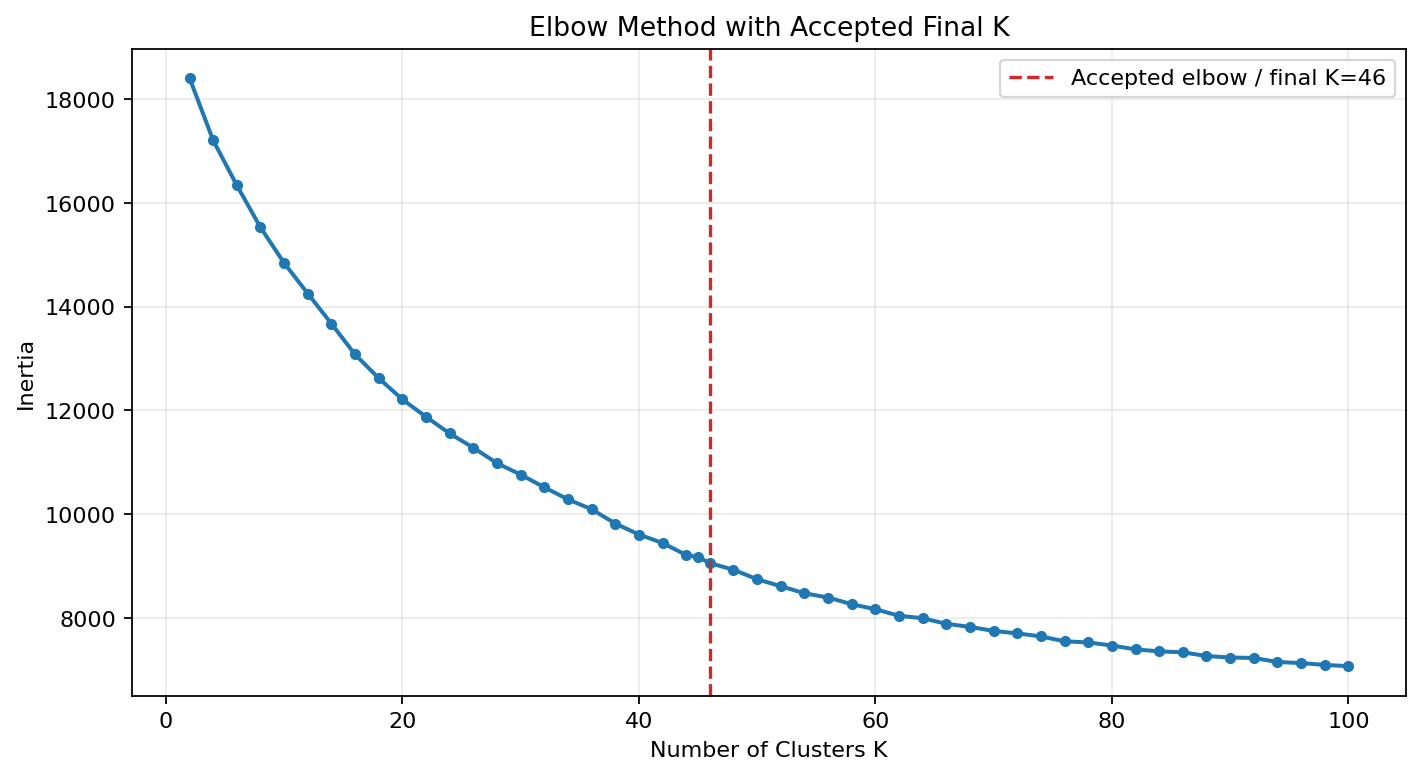
\includegraphics[width=\linewidth]{../outputs/figures/kneedle_elbow.png}
\end{minipage}\hfill
\begin{minipage}{0.48\textwidth}
\centering
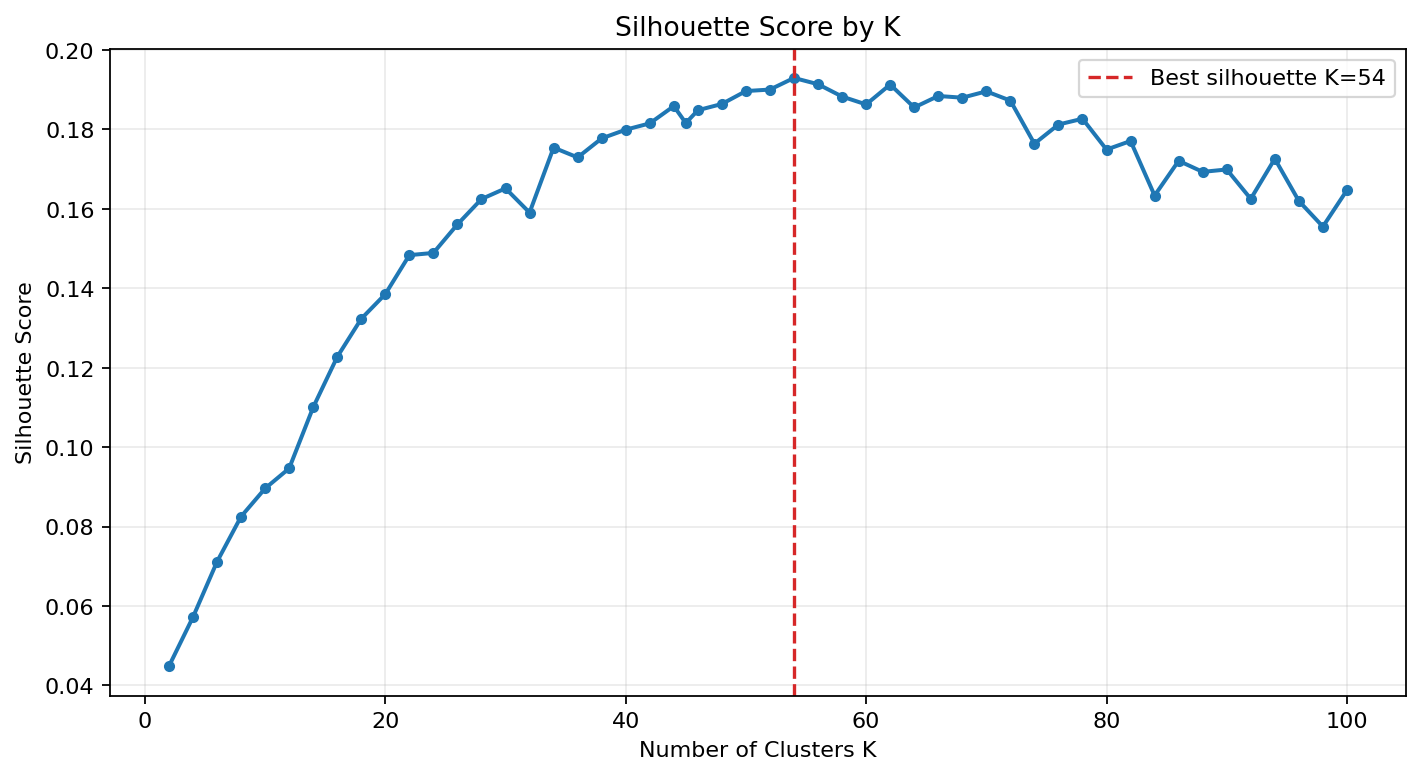
\includegraphics[width=\linewidth]{../outputs/figures/silhouette_scores.png}
\end{minipage}

\vspace{0.4cm}

\begin{minipage}{0.48\textwidth}
\centering
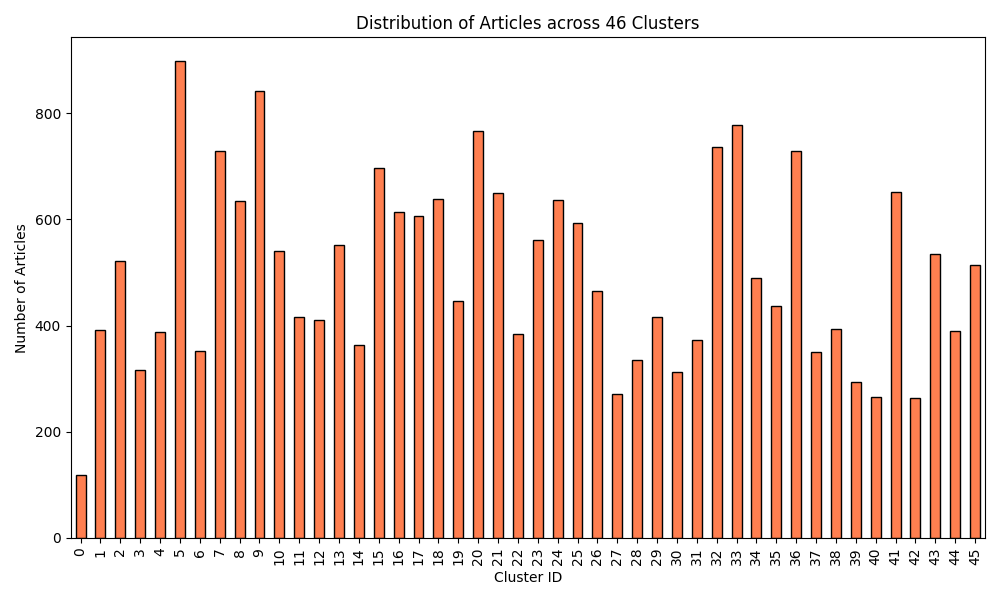
\includegraphics[width=\linewidth]{../outputs/figures/cluster_distribution.png}
\end{minipage}\hfill
\begin{minipage}{0.48\textwidth}
\centering
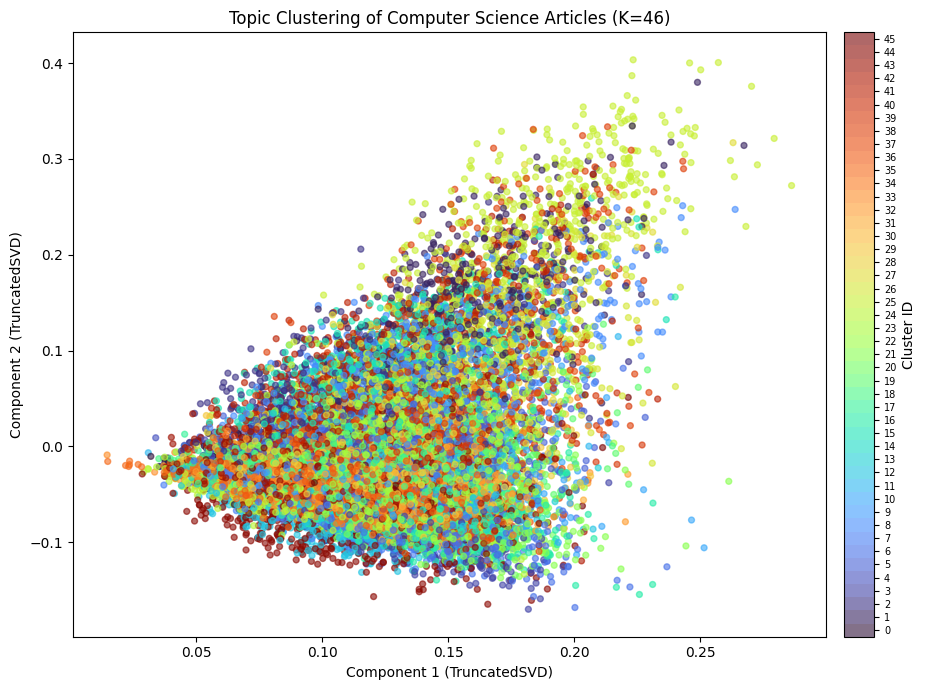
\includegraphics[width=\linewidth]{../outputs/figures/cluster_visualization.png}
\end{minipage}
\caption{Final visual outputs. Top-left: elbow / inertia curve with the accepted final choice. Top-right: silhouette score across the broad $K$ sweep. Bottom-left: article counts per cluster for the accepted $K=46$ model. Bottom-right: two-dimensional Truncated SVD projection of the final clustered feature space.}
\label{fig:visuals}
\end{figure*}

\section{Conclusion}
The final delivery satisfies the homework objectives while presenting a cleaner and more defensible clustering decision process. The recommendation stage remains a strong classical baseline with solid hold-out performance. The clustering stage now documents a broad $K$ search, retains the accepted elbow-based $K=46$ decision, and clearly distinguishes the final K-Means solution from the experimental BERTopic alternatives.

The final choice favors reproducibility, interpretability, and a lightweight submission over a heavier experimental topic-modeling stack. This makes the delivered project easier to run, easier to explain, and better aligned with the homework requirement of producing a practical journal finder and topic clustering system.

\begin{thebibliography}{00}
\bibitem{cbf_recommender} P. Lops, M. de Gemmis, and G. Semeraro, ``Content-based Recommender Systems: State of the Art and Trends,'' in \textit{Recommender Systems Handbook}, Springer, 2011, pp. 73--105.
\bibitem{metadata_nlp} X. Wang et al., ``A literature review on academic recommender systems,'' \textit{Information Processing \& Management}, vol. 54, no. 6, pp. 883--912, 2018.
\bibitem{journal_scoring} S. Sugiyama and M. Kan, ``Scholarly Paper Recommendation via User's Recent Research Interests,'' in \textit{Proc. of the 10th ACM/IEEE-CS Joint Conference on Digital Libraries}, 2010.
\bibitem{kmeans_svd} C. D. Manning, P. Raghavan, and H. Sch\"utze, \textit{Introduction to Information Retrieval}, Cambridge University Press, 2008.
\end{thebibliography}

\end{document}
